%% jbc-template.tex, version 1.0, 2016/08/16
\documentclass[alpha-refs]{wiley-article}
% \documentclass[blind,num-refs]{wiley-article}

% Add additional packages here if required
\usepackage{siunitx}

% Update article type if known
\papertype{Original Article}
% Include section in journal if known, otherwise delete
\paperfield{Methods & Resources}
\usepackage{graphicx}

% These packages can be used!
\usepackage{amsmath,amssymb,mathtools}
\usepackage[version=3]{mhchem}
\usepackage{siunitx}
\usepackage[colorlinks=true, allcolors=blue]{hyperref}

\title{Batch effects in large-scale proteomics studies: diagnostics and correction}

\runningtitle{Batch effects in large-scale proteomics studies: diagnostics and correction}

% Use \authormark if required to clarify multiple institutions
\author{Jelena Čuklina\authormark{1, 2, 3}, Chloe Lee\authormark{1}, Evan G. Williams\authormark{1}, Tatjana Sajic\authormark{1}, Ben C. Collins\authormark{1}, Maria Rodriguez-Martinez\authormark{3}, Varun Sharma\authormark{1}, Patrick Pedrioli\authormark{1, 4}, Ruedi Aebersold\authormark{1, 5}}

\affil{\authormark{1}Institute of Molecular Systems Biology, ETH Zurich, Zurich, CH-8093, Switzerland,\authormark{2} PhD Program in Systems Biology, University of Zurich and ETH Zurich,
Zurich, CH-8057  Switzerland, \authormark{3} IBM Zurich Research Laboratory, Rüschlikon, CH-8803, Switzerland, \authormark{4}ETH Zürich, PHRT-MS, Zürich, Switzerland, \authormark{5}Faculty of Science, University of Zurich, Zurich, Switzerland}

\corr{Ruedi Aebersold, +41 44 633 31 70 \email{aebersold@imsb.biol.ethz.ch} }

\keywords{Batch effects, Quantitative proteomics, Normalization, Preprocessing,}

\begin{document}

\maketitle

\begin{article}
\begin{abstract}
\textit{The abstract should succinctly and clearly describe the major findings reported in the manuscript. It must not exceed 250 words.}

Recent technical advances in mass spectrometry based proteomics have significantly increased robustness, sample throughput and sample to sample reproducibility to a degree that large-scale studies consisting of hundreds of samples are becoming routine. Whereas, increased sample numbers facilitate statistical association of proteome states with phenotypes, they generally come at the price of introducing batch effects, that decrease the power to identify the underlying biological variance. Bottom-up proteomics is a multistep process, consisting of biosample collection, protein digestion and mass-spectra acquisition. Each of the steps can result in batch effects, that need to be accounted for before biological signal inference.
Here, we  describe a step-by-step workflow that allows to identify batch effects, select appropriate methods for their correction and control the quality of the correction. We present a corresponding tool, a novel R package "proBatch" that implements each of the steps. 
We also address several mass-spectrometry specific issues, associated with batch effects. First, we demontstrate MS signal deterioration, associated with sample running order. To address it, we propose a new correction procedure based on LOESS trend fitting. Then, we highlight the issue of batch-specific missingness patterns and discuss the problem of missing value imputation in the context of batch effects.
We demonstrate the workflow and the package using three large  proteomics datasets, spanning 140-375 mass-spectromentry runs, representing different biological backgrounds and sources of batch effects. Although applied to DIA proteomics, the principles described here are expected to be applicable to wide range of proteomic methods.

 

\end{abstract}

\textit{The introduction begins after the abstract and is not preceded by the word ``Introduction.''}

The introduction presents the purpose of the study and its relationship to earlier work in the field. It should not be an extensive review of the literature. It is usually less than one formatted page

\section{Results}

The results should be presented in figures, tables, or text. Figures (e.g. Figure \ref{fig:july29cover}) and tables (e.g. Table \ref{tab:sample}) are displayed in order after the main article text. Figure and table legends will appear immediately after the corresponding figure or table.

\begin{figure}[hbtp!]\centering
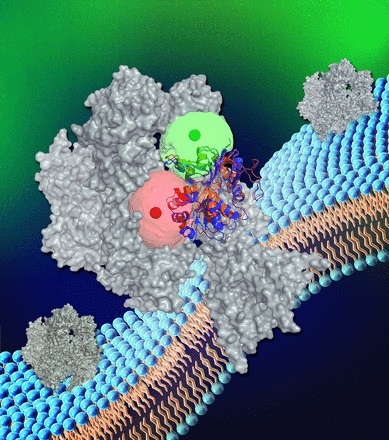
\includegraphics[width=0.5\textwidth]{figures/jbc-cover-20160729.jpg}
\caption{Sample Figure (July 29, 2016 JBC issue cover).}
\label{fig:july29cover}
\end{figure}

\begin{figure}[hbtp!]\centering
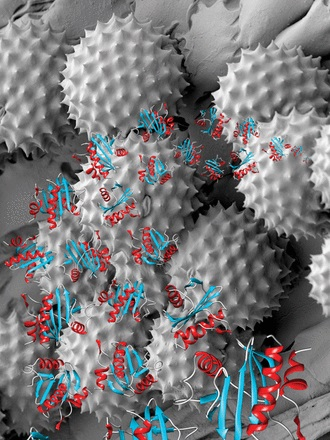
\includegraphics[width=0.5\textwidth]{figures/jbc-cover-20160722.jpg}
\caption{Sample Figure (July 22, 2016 JBC issue cover).}
\label{fig:july22cover}
\end{figure}

\begin{table}[hp!]\centering
\begin{tabular}{l r r}
Sample Heading 1 & Sample Heading 2 & Sample Heading 3\\
\hline
Data 1 & 3.8 & 0.12 \\
Data 2 & 49.2 & 0.52
\end{tabular}
\caption{A Sample Table}
\label{tab:sample}
\end{table}

References, such as \cite{macdonald1995difference,sambrook1989molecular,waskiewicz1997mitogen,back:etal:2017}, must be cited in text by number only, be numbered consecutively in the order of appearance, and must include article titles, as in these examples. 

Reference management systems such as Zotero and Mendeley provide options for exporting bibliographies as Bib\TeX{} files. Bib\TeX{} is a bibliographic tool that is used with \LaTeX{} to help organize the author's references and create a bibliography. This template contains an example of such a file, \texttt{sample.bib}, which can be replaced with your own. Use the \verb|\cite| command  to create in-text citations.

\section{Discussion}

The discussion is concise (usually less than two formatted pages) and focused on the interpretation of the results. It should not repeat information in the ``Results'' section.

\section{Experimental Procedures}

The experimental procedures are brief but sufficiently complete to permit a qualified reader to repeat the experiments. Only truly new procedures should be described in detail. Previously published procedures should be referenced. Modifications of previously published procedures should not be given in detail except where necessary to repeat the work. If the study characterizes the activity of new compounds, compound structures must be provided. Quantification of gel or blot intensities must be performed with data obtained within a linear range of exposure.

\end{article}

\begin{acknowledgments}
Acknowledgments may include funding sources, brief note(s) of thanks to people who helped with the study or preparation of the paper (optional), and database names and accession codes (if applicable). 
\end{acknowledgments}

\begin{conflict}
Statement disclosing whether there are any actual or perceived conflicts of interest on the part of any author. If there are no conflicts of interest, insert the following statement: The authors declare that they have no conflicts of interest with the contents of this article. Review the “Conflicts of interest” section of the \href{http://www.jbc.org/site/misc/edpolicy.xhtml}{JBC Editorial Policies}.
\end{conflict}

%% Bibliography 
\bibliographystyle{jbc-new}
\bibliography{sample}

\begin{footnotes}
Footnotes should include details such as grant information, and any abbreviations used within the article.
\end{footnotes}

\end{document}
